\chapter{Introduction}
This report and the corresponding documentation with its appendix is written as the documentation of the development process for the AU2 car, the dynamometer dubbed Rolling Road and the GUI developed for use with the Rolling Road. The products being developed are made to compete in the Shell Eco Marathon. The development process is accomplished in correlation with Aarhus School of Engineering(ASE). The development is part of the 4. semester project. 

This report covers three major subjects:

\begin{itemize}
	\item{AU2}
	\item{Rolling Road}
	\item{GUI}
\end{itemize}

AU2 is the car built to compete in the Shell Eco-Marathon. In this report the electrical systems developed for controlling the car will be described. For more information containing calculations and general knowledge about the physical implementation of the car please visit the technical documentation.

The Rolling Road and GUI is a coherent system, though they can function independently. This report will only cover the electrical system developed along with the software, both for Rolling Road and the GUI. 

This report will only scratch the surface. For in-depth design and implementation features, please visit the associated documentation\fxnote{det står også ved AU2 - måske undlade denne sætning og generalizere den ved AU2, eller slette det ved AU2 også lade denne blive... LB}. 

The products being developed will serve as a working product that has been thoroughly tested. This is done so that no breakdown occurs during the race. It will also work as a guideline for future work for other students that will work with the SEM. Therefore it is necessary that the documentation provided alongside this report must be comprehensive.\fxnote{skriv noget om at vi har arbejdet sammen me m-ingeniøre}
\fxnote{kan vi skrive noget om hvorfor vi valgte at skrive på engelsk}

\section{List of terms}
The following list explains the various terms which is used in this report to refer to various relevant items from all three systems:
\begin{itemize}
	\item \textbf{SEM}\\
	The Shell Eco-Marathon 2016 which is held at London and which one of the goals of this project has been to compete in.
	\item \textbf{AU - Shell Eco Marathon Team}\\
	The complete team consisting of both electrical and mechanical engineers who developing AU2 in order to compete in Shell Eco-Marathon.
	\item \textbf{PSoC}\\
	Refers to the CY8CKIT-059 PSoC 5LP Prototype Kit which is used to build the Control Unit in Rolling Road and the Motor Controller in AU2.
	\item \textbf{Zenith33}\\
	A electrically propulsed car which had been designed to compete in Shell Eco-Marathon 2014\cite{BAC_zenith33} on behalf of AU. Due to its design, this car was not allowed to compete in SEM 2016. However, due to the mechanical body of AU2 being developed in parallel many of the tests were performed using Zenith33.
	\item \textbf{Previous dynamometer}\\
	An earlier version of Rolling Road called 'Teststand tilBørsteløs DC Motor'\cite{BAC_rullefelt}. 
\end{itemize}

\fxnote{Vil skal lige huske og at tilføje nogle på et tidspunkt, som AU2 og SEM - JH}

\section{Reading guide}

This report gives the reader an insight into the different aspects of developing this project, such as the key documentation to gain an overview of the system and some of the challenges met while developing.

The report can be split into multiple parts:

\textbf{First part} of the report gives a quick overview of the system and the team-members who helped develop the system. It includes chapter 1 through 4.

\textbf{Second part} describes the process used to manage the project and programs used to in the development process, and includes chapter 5 and 6.

\textbf{Third part} describes the requirements, overall architecture and the design considerations, implementation and test of different systems developed as a part of this project.  and includes chapter 7 through 10

\textbf{Fourth part} includes chapter 11 and 12 and talks about the results, what could be done in the future to enhance the product and lastly some of the experience gained, both as a group and individually for each team member.

\textbf{Fifth part} concludes the project as a whole and consists of chapter 14

\clearpage
\section{Areas of responsibility}
In the following table the team members will describe their primary responsibilities during the project. 

\begin{tabular}[c]{|p{3cm}| p{5cm} | p{6cm}|}
	\hline
	\textbf{Member} & \textbf{Area of responsibility} & \textbf{Description}\\\hline
	
	% Jens
	\phantom{Test}
	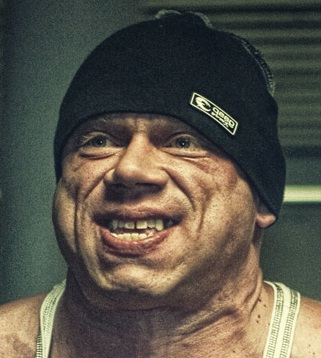
\includegraphics[width=3cm]{Introduction/TeamPictures/Jens} & \multirow{2}{5cm}{Area of responsibility goes here} & \multirow{2}{6cm}{Description goes here plzzzzzzzzzzzzzzzz} \\
	Jens P. Nymann & & \\ \hline
	
	%Jonas
	\phantom{Test}
	
\includegraphics[width=3cm]{Introduction/TeamPictures/Jonas} & \multirow{2}{5cm}{SCRUM-Master and software developer on the Rolling Road GUI and AU2} & \multirow{2}{6cm}{As the SCRUM-master i've been in charge of the bi-weekly SCRUM standup meetings and planning of new sprints.\\
		I was also in charge of the Rolling Road GUI Application and in addition wrote the SD-Card logging software for the AU2.
		} \\
	Jonas M. Hansen & & \\ \hline
	
	%Jonathan
	\phantom{Test}
	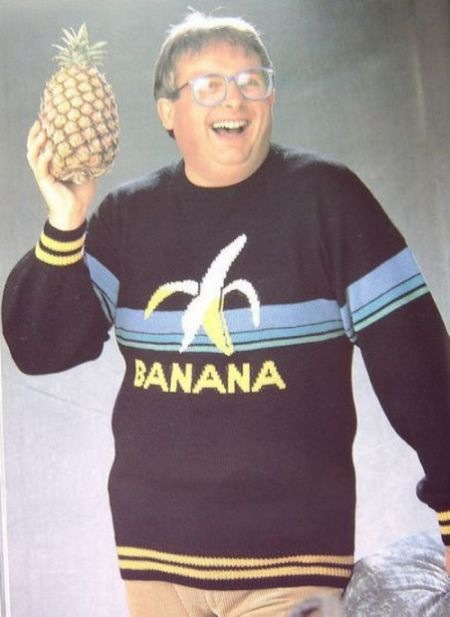
\includegraphics[width=3cm]{Introduction/TeamPictures/Jonathan} & \multirow{2}{5cm}{Area of responsibility goes here} & \multirow{2}{6cm}{Description goes here plzzzzzzzzzzzzzzzz} \\
	Jonathan Schougaard & & \\ \hline
\end{tabular}

\newpage
\begin{tabular}[c]{|p{3cm}| p{5cm} | p{6cm}|}
	\hline
	\textbf{Member} & \textbf{Area of responsibility} & \textbf{Description}\\\hline
	
	%Laimonas
	\phantom{Test}
	
\includegraphics[width=3cm]{Introduction/TeamPictures/Laimonas} & \multirow{2}{5cm}{eating and BMS changes allll around... ignore - fixed later halp} & \multirow{2}{6cm}{Description goes here plzzzzzzzzzzzzzzzz, no} \\
	Laimonas I. \newline Bendikas & & \\ \hline
		
	%Thomas R
	\phantom{Test}
	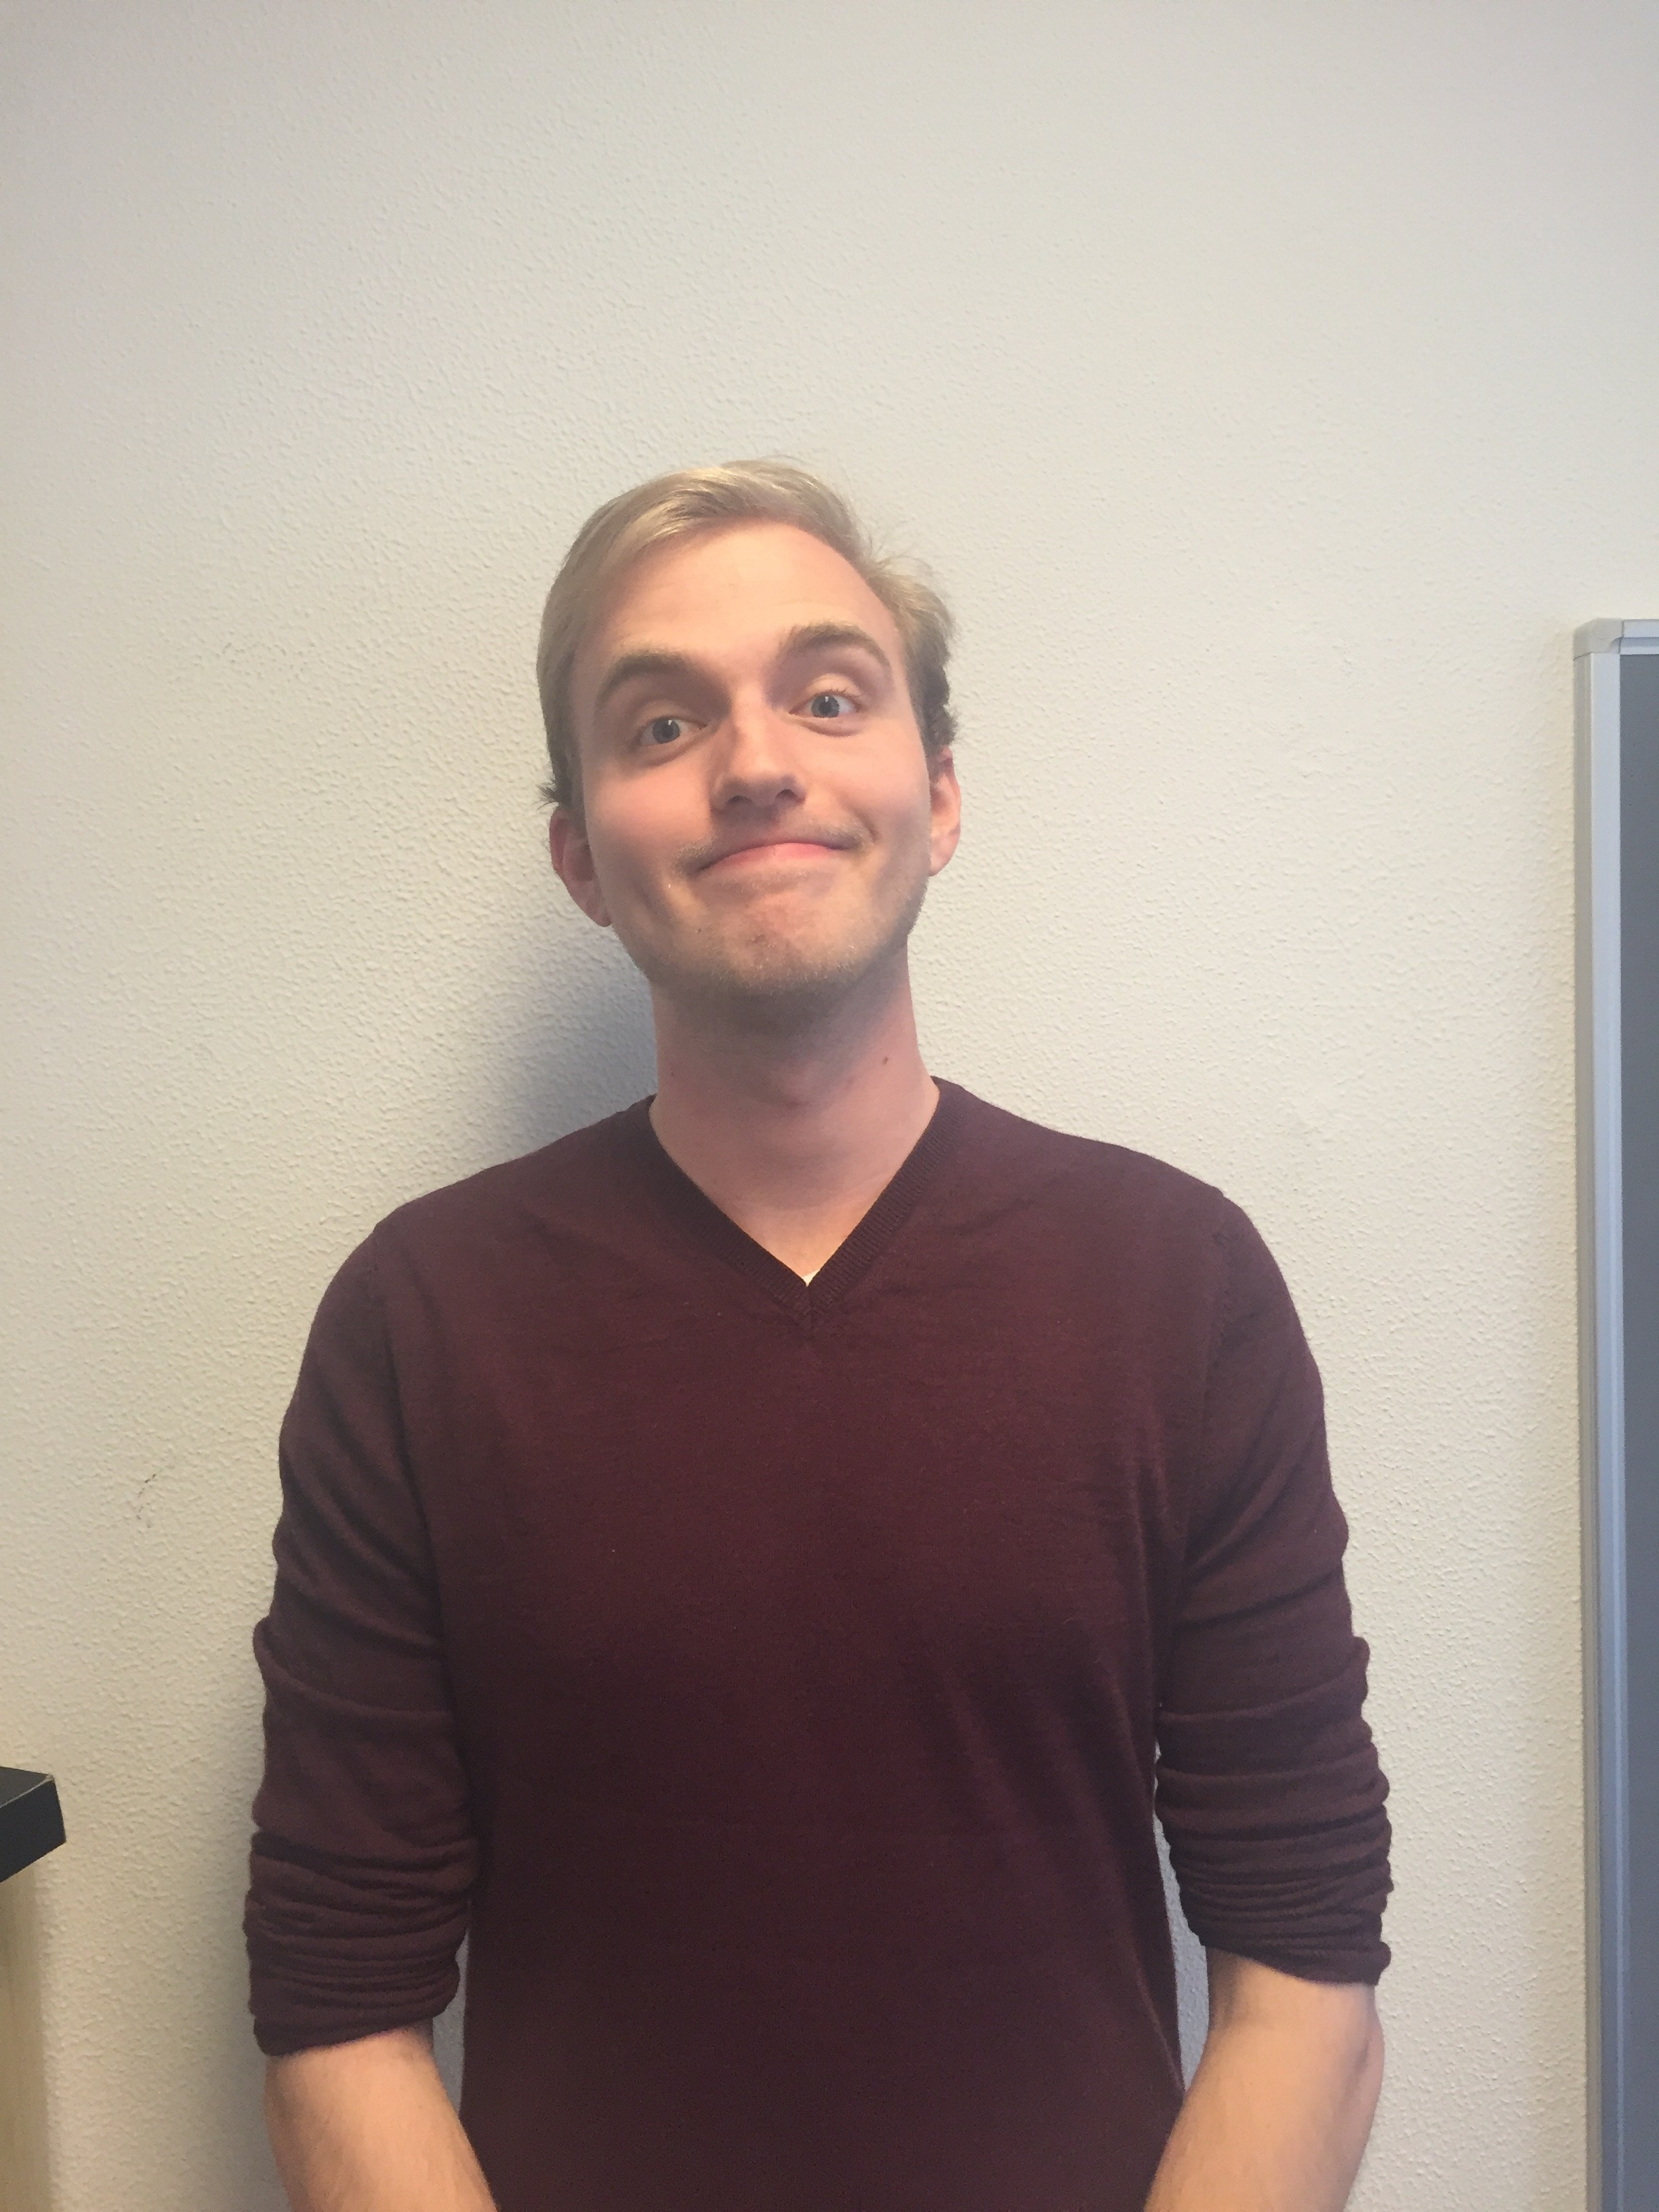
\includegraphics[width=3cm]{Introduction/TeamPictures/ThomasR} & \multirow{2}{5cm}{Architecture on both Rolling Road and AU2.\newline \newline Hardware analysis, design and implementation on Rolling Road.} & \multirow{2}{6cm}{I've been responsible for creating the system-descriptions of both Rolling Road and AU2 and their individual architectures.\newline \newline Furthermore, i have been responsible for analysing the previous dynamometer-system in order to create the hardware in Rolling Road.} \\
	Thomas S. \newline Rasmussen & & \\ \hline
		
	%Thomas N
	\phantom{Test}
	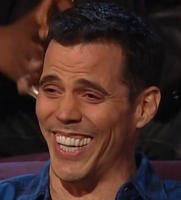
\includegraphics[width=3cm]{Introduction/TeamPictures/ThomasN} & \multirow{2}{5cm}{Hardware development for AU2 \newline \newline Protocol development for RR} & \multirow{2}{6cm}{I have been responsible for the design and implementation of the hardware for AU2. Furthermore I have developed the Protocol for Rolling Road} \\
	Thomas B. \newline Nielsen & & \\ \hline
\end{tabular}